\documentclass[12pt]{article}
\usepackage[utf8]{inputenc}
\usepackage[english]{babel}
\usepackage[dotinlabels]{titletoc}
\usepackage{mathptmx}
\usepackage{amsmath, amssymb}
\usepackage{geometry, titlesec, setspace, enumitem}
\usepackage{xcolor, graphicx, caption, subcaption}
\usepackage{hyperref, natbib}
% Journals
\newcommand{\aap}{A\&A}
\newcommand{\aj}{AJ}
\newcommand{\apj}{ApJ}
\newcommand{\araa}{ARA\&A}
\newcommand{\mnras}{MNRAS}
\newcommand{\nat}{Nature}
\newcommand{\pasa}{PASA}
\newcommand{\pasp}{PASP}
\newcommand{\physrep}{PhR}
\newcommand{\prd}{PhRvD}
\newcommand{\rpph}{RPPh}

% Page formatting
\geometry{
	left=1.25in,
	right=1.25in,
	top=1in,
	bottom=1in}
\hypersetup{
	colorlinks=true,
	citecolor=blue,
	filecolor=blue,
	linkcolor=blue,
	urlcolor=blue
}
\setlength{\footnotesep}{10pt}
\setlist{noitemsep}

% Fixing titlesec and hyperref interaction
\makeatletter
\def\ttl@useclass#1#2{%
\@ifstar
{\ttl@labeltrue\@dblarg{#1{#2}}}
{\ttl@labeltrue\@dblarg{#1{#2}}}}
\makeatother

% Image setup
\graphicspath{{figs/}}
\captionsetup[figure]{labelfont={bf}, font={small, stretch=1.3}, name={Figure}, labelsep=period}

% Section and subsection headings
\titleformat{\section}{\normalsize\bfseries\centering}{}{0em}{}
\titleformat{\subsection}{\normalsize\itshape\centering}{}{0.75em}{}
\newcommand{\nocontentsline}[3]{}
\newcommand{\tocless}[2]{\bgroup\let\addcontentsline=\nocontentsline#1{#2}\egroup}
\renewcommand{\contentsname}{Table of Contents}
\renewcommand{\abstractname}{{\normalsize\bfseries\centering{Abstract}}}
\renewcommand{\bibsection}{}

% For figures
\makeatletter
\setlength{\@fptop}{0pt plus 1fil}
\setlength{\@fpbot}{0pt plus 1fil}
\makeatother

% For formatting text and math
\let\vec\mathbf
\newcommand{\code}[1]{{\fontfamily{qcr}\selectfont#1}}
\newcommand{\red}[1]{\textcolor{red}{#1}}
\newcommand{\note}[1]{\textcolor{violet}{#1}}

% Special commands
\newcommand{\HI}{H\,\textsc{i}}
\newcommand{\OI}{O\,\textsc{i}}
\newcommand{\heraqm}{\code{hera\textunderscore qm}}
\newcommand{\herapspec}{\code{hera\textunderscore pspec}}
\newcommand{\herasim}{\code{hera\textunderscore sim}}
\newcommand{\pyuvdata}{\code{pyuvdata}}

\begin{document}
\doublespacing
\begin{center}
Environmental Systematics and the Impact on \\ 21-cm Epoch of Reionization Measurements \\
by \\
Lily Whitler \\
has been approved \\
Spring 2019 \\[0.1\textheight]

\begingroup
\renewcommand{\arraystretch}{0.7}
\begin{tabular}{p{1cm}p{3.5in}p{1cm}}
	& \centering APPROVED: & \\
	& & \\ & & \\
	& \hrulefill & \\
	& \hfill Daniel Jacobs, Director & \\
	& & \\ & & \\
	& \hrulefill & \\
	& \hfill Judd Bowman & \\
	& & \\ & & \\
	& \hrulefill & \\
	& \hfill Adam Beardsley &
\end{tabular} \\[0.075\textheight]
\begin{tabular}{p{1cm}p{3.5in}p{1cm}}
	& \centering ACCEPTED: & \\
	& & \\ & & \\
	& \hrulefill & \\
	& \hfill Dean, Barrett, The Honors College &
\end{tabular}
\endgroup
\end{center}
\thispagestyle{empty}
\newpage
\pagenumbering{arabic}

\begin{center}
	Environmental Systematics and the Impact on \\ 21-cm Epoch of Reionization Measurements \\
	by \\
	Lily Whitler \\[0.15\textheight]
	
	A Thesis Presented in Partial Fulfillment \\
	of the Requirements for Graduation from \\
	Barrett, the Honors College \\[0.15\textheight]
	
	Committee: \\
	Daniel Jacobs, Director \\
	Judd Bowman \\
	Adam Beardsley \\[0.23\textheight]
	
	ARIZONA STATE UNIVERSITY \\
	April 2019
\end{center}
\thispagestyle{empty}

\clearpage
\pagenumbering{roman}

\begin{center}
	\textbf{Abstract}
\end{center}

The Epoch of Reionization (EoR) is the period in the evolution of the universe during which neutral hydrogen was ionized by the first luminous sources, and is closely linked to the formation of structure in the early universe. The Hydrogen Epoch of Reionization Array (HERA) is a radio interferometer currently under construction in South Africa designed to study this era. Specifically, HERA is dedicated to studying the large-scale structure during the EoR and preceding Cosmic Dawn by measuring the redshifted 21-cm line from neutral hydrogen. However, the 21-cm signal from the EoR is extremely faint relative to galactic and extragalactic radio foregrounds, and additional instrumental and environmental systematics make measuring the signal all the more difficult. Radio frequency interference (RFI) from terrestrial sources is one such systematic. In this thesis, we explore various methods of removing RFI from early science-grade HERA data and characterize the effects of different removal patterns on the final 21-cm power spectrum. In particular, we focus on the impact of masking narrowband signals, such as FM radio and aircraft or satellite communications, in the context of the algorithms currently used by the HERA collaboration for analysis. 

\newpage
\begingroup
\hypersetup{
	citecolor=DarkBlue,
	filecolor=black,
	linkcolor=black,
	urlcolor=DarkBlue
}
\renewcommand{\thesection}{\Roman{section}}
\tableofcontents
\listoffigures
\endgroup

\newpage
\begin{center}
	\textbf{Acknowledgements}
\end{center}

First and foremost, thank you to my many research mentors past and present for their time and teaching, especially (in no particular order) Adam Beardsley, Judd Bowman, Danny Jacobs, and Rogier Windhorst. In particular, I would like to extend my sincere gratitude to Adam for his mentorship, advice, knowledge, critiques, and general support. I owe a large part of my interest in and knowledge of radio astronomy to him. Thank you to my fellow undergraduates in the ASU HERA group and Rogier Windhorst's cosmology group; my particular appreciation goes to Shane Bechtel, Tyler Cox, and Cameron White for their advice, assistance, conversations, and friendship, all of which greatly enhanced this work and my enjoyment of it. And finally, last but certainly not least, thank you to my parents and sisters for their constant support and encouragement.

This material is based upon work supported by the National Science Foundation under Grant No. 1636646, the Gordon and Betty Moore Foundation, and institutional support from the HERA collaboration partners. HERA is hosted by the South African Radio Astronomy Observatory, which is a facility of the National Research Foundation, an agency of the Department of Science and Technology.

\clearpage
\pagenumbering{arabic}

\tocless\section{\hypertarget{sec:introduction}{1.\hspace{0.75em}Introduction}}
\addcontentsline{toc}{section}{1.\hspace{0.75em}Introduction}

\tocless\subsection{\hypertarget{subsec:universe}{1.1.\hspace{0.75em}A Brief History of the Universe}}
\addcontentsline{toc}{subsection}{1.1.\hspace{0.75em}A Brief History of the Universe}

Immediately after the Big Bang, the universe was a hot plasma of fundamental particles. Now, nearly 14 billion years later, it is populated with a rich variety of objects and structure, from massive galaxy clusters all the way down to our own solar system and its planets. However, there is an important piece missing: we know what the very young universe looked like, and we know what it looks like today, but the evolutionary path it took from then to now is not entirely clear.

In the early universe, matter was hot and ionized. Photons scattered off of free particles, rendering the universe opaque to electromagnetic radiation. This lasted until approximately 380,000 years after the Big Bang, at which point the universe had expanded and cooled sufficiently for electrons to become bound to atomic nuclei during recombination. When recombination was complete, photons were able to propagate freely through space, subject only to cosmological redshift. Today, we see photons from this era as the cosmic microwave background (CMB).

Immediately following the release of the CMB and lasting until several hundred million years after the Big Bang was the cosmic Dark Ages. During this era, though photons were free to propagate through space, no stars, galaxies, or other sources of radiation had yet formed. The only sources of information we have from the Dark Ages are CMB photons and emission from neutral hydrogen.

The transition between the Dark Ages and the subsequent Epoch of Reionization (EoR) was marked by the emergence of the first luminous sources. During the EoR, ultraviolet (UV) radiation from these objects ionized the intergalactic medium (IGM) around them. The EoR ended when the IGM was fully ionized, thus completing the final major phase change of hydrogen in the universe.

Figure \ref{fig:timeline} shows an illustration of this evolution. The \textit{Planck} satellite and its predecessors, the \textit{Cosmic Background Explorer} and \textit{Wilkinson Microwave Anisotropy Probe}, have measured the anisotropies in the CMB, providing a wealth of information about the universe just a few hundred thousand years after the Big Bang. On the other end of cosmic history, deep imaging and spectroscopic observations with ground- and space-based telescopes have probed some of the oldest known galaxies. However, most of the Dark Ages and EoR still lack observational constraints. \vspace{3mm}

\begin{figure}[tb]
	\centering
	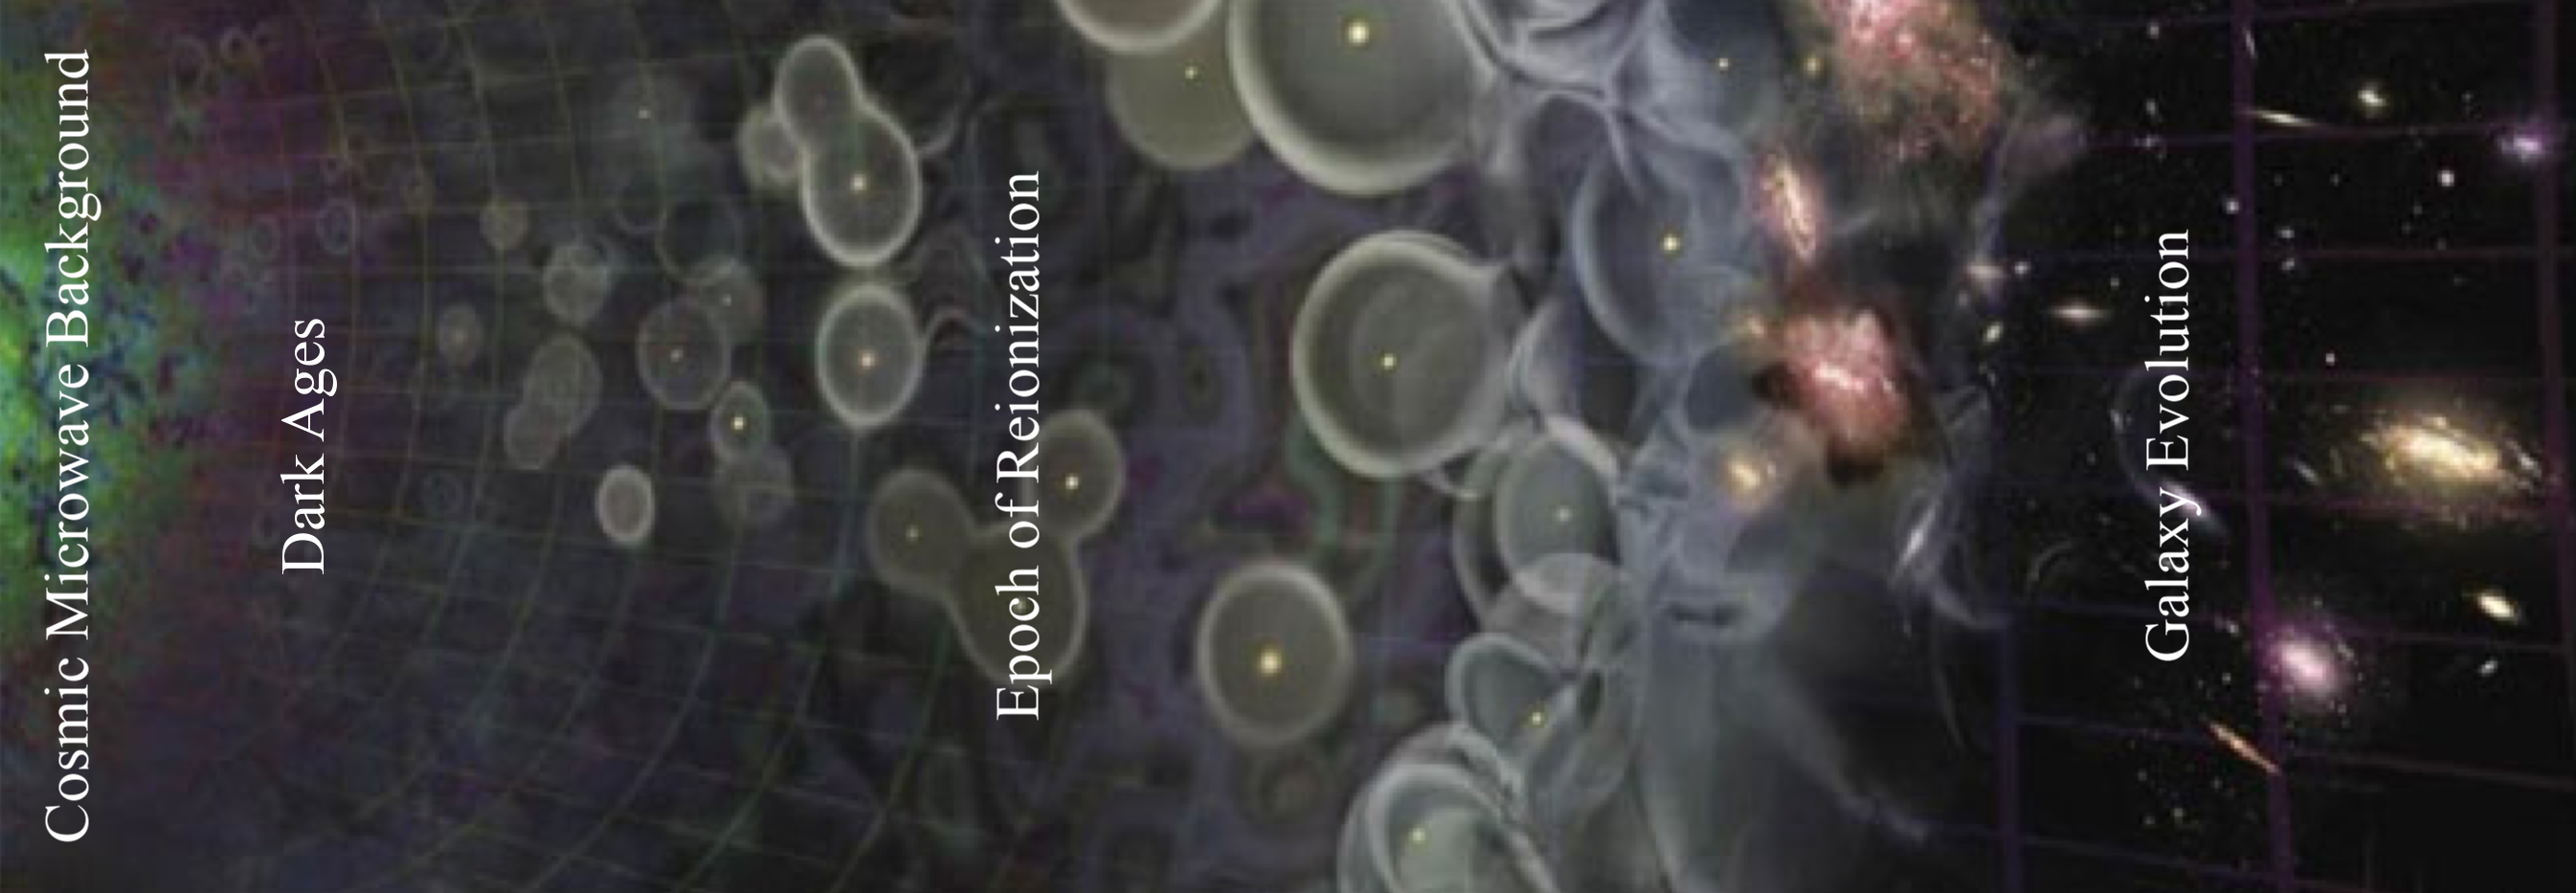
\includegraphics[width=\textwidth]{timeline.png}
	\caption[History of the universe]{A visualization of cosmic evolution. Image modified from \cite{loeb2006}.}
	\label{fig:timeline}
\end{figure}

\tocless\subsection{\hypertarget{subsec:eor}{1.2.\hspace{0.75em}The Epoch of Reionization}}
\addcontentsline{toc}{subsection}{1.2.\hspace{0.75em}The Epoch of Reionization}

\begin{figure}[t]
	\centering
	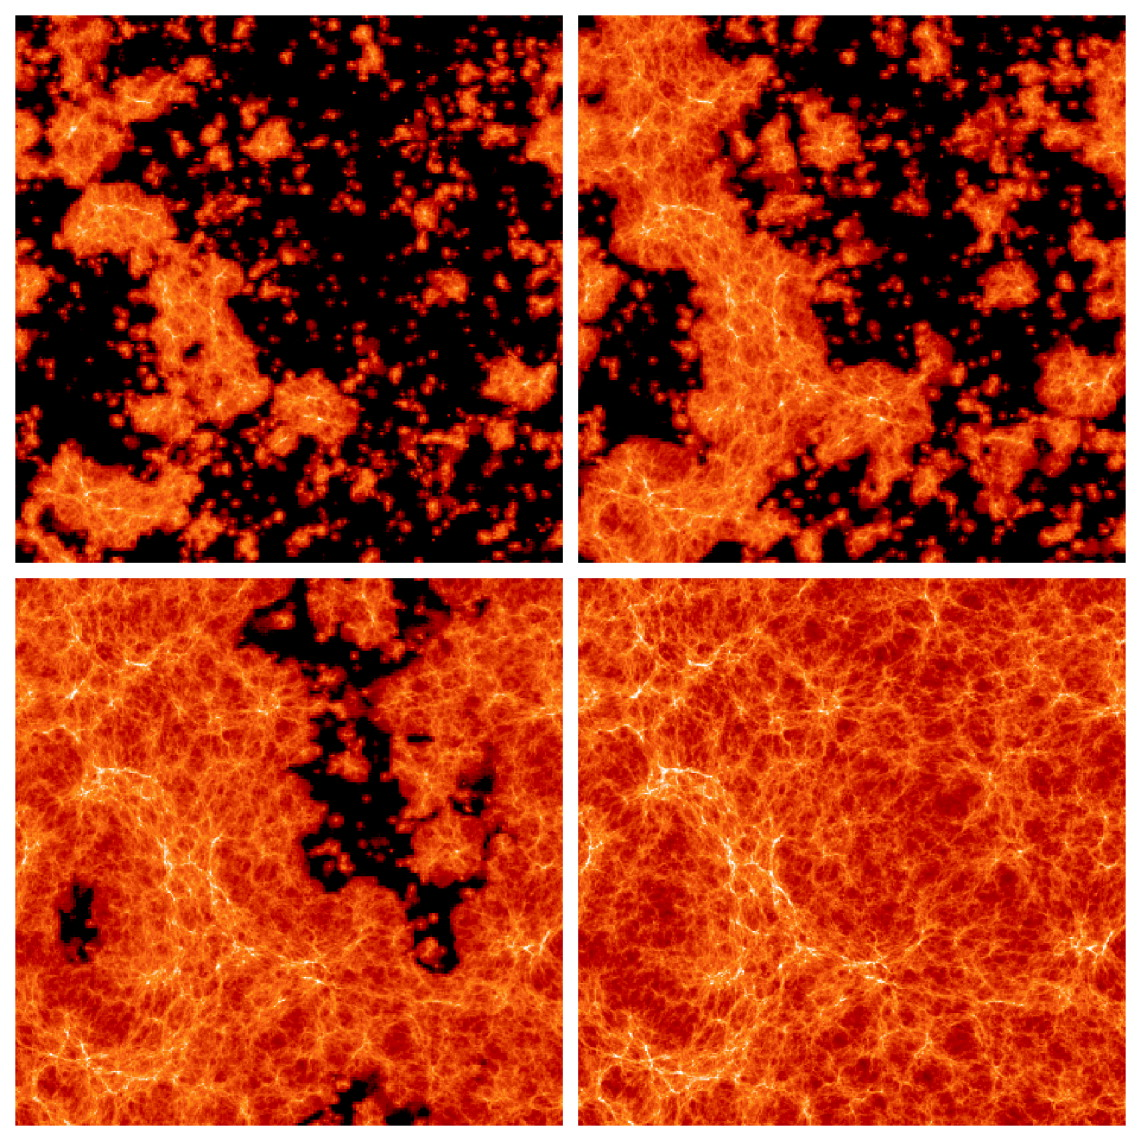
\includegraphics[width=0.75\textwidth]{reionization_slices.jpg}
	\caption[Redshift slices through a simulation showing the evolution of ionized hydrogen]{Slices through a reionization simulation showing the density of ionized hydrogen at redshifts 9 (top left), 8 (top right), 7 (bottom left), and 6 (bottom right). Image from \cite{trac2007}.}
	\label{fig:reionization}
\end{figure}

The EoR is the period in cosmic history during which the hydrogen in the universe, which had been neutral since recombination, was ionized by the very first luminous sources. Studying this era, along with the Dark Ages, will provide the bridge between the CMB and the universe today.

Though the EoR is largely observationally unconstrained, theoretical studies have constructed a broad picture of the ionization process. UV photons from the earliest energetic sources ionized the gas in their immediate neighborhood, and as individual objects continued ionizing their surroundings, these bubbles of ionized gas grew in size and eventually began to overlap. As the EoR progressed, this process of growing ionized bubbles continued until the IGM was fully ionized and only pockets of neutral hydrogen in galaxies remained. Figure \ref{fig:reionization} shows a simulated visualization of this evolution.

This qualitative picture is generally accepted, and is even fairly intuitive. However, understanding the quantitative details such as the timeline, topology, and the nature of the first luminous sources will require observations. \vspace{3mm}

\tocless\subsection{\hypertarget{subsec:constraints}{1.3.\hspace{0.75em}Observational Constraints on the Epoch of Reionization}}
\addcontentsline{toc}{subsection}{1.3.\hspace{0.75em}Observational Constraints on the Epoch of Reionization}

One observational approach currently being undertaken is via the ionizing sources. \cite{fan2006} constrained the end of reionization to be no later than $z \sim 6$, primarily via observations of the Gunn-Peterson trough in spectra of high-redshift quasars. In the future, this approach will continue to place tighter limits on the end of reionization, especially since deep surveys with the upcoming \textit{James Webb Space Telescope} and other ground- and space-based instruments will enable detections of statistical samples of these high-redshift objects. However, the number of detected quasars at $z \gtrsim 7$ to date is not large, and there is evidence that the quasar luminosity function drops off at these redshifts, thus limiting our ability to study the earlier part of the EoR with these objects \citep{richards2006, hopkins2007}.

Other probes of the EoR include gamma ray bursts and metal absorption line systems. High-redshift gamma ray bursts exhibit troughs blueward of Lyman-alpha in their spectra due to absorption by intervening neutral hydrogen; this allows them to serve as a probe of the ionization state of the IGM \citep[e.g.,][]{gallerani2008}. Early star formation enriches the interstellar medium and the IGM with heavy elements. The emission lines from these elements can be used either to probe the properties of the stellar populations that ionized the universe or to directly trace the ionization history. For example, \cite{oh2002} proposed the using the \OI~line at 1302 \AA~as a tracer of the neutral fraction of hydrogen, since \OI~and H have almost identical ionization potentials and \OI~is expected to be in tight charge exchange equilibrium with H.

Both the large-scale polarization of the CMB and the small-scale kinetic Sunyaev-Zel'dovich (kSZ) effect place some constraints on the onset and topography of reionization \citep{fan2006}. CMB photons undergo Thomson scattering off of free electrons produced by the ionization of hydrogen, which causes the emission to linearly polarize at horizon scale. This suppresses primary CMB anisotropies, so measuring the polarization constrains the onset of the EoR \citep[e.g.,][]{zaldarriaga1997, roy2018}. The kSZ effect, on the other hand, is due to inverse Compton scattering of ionized electrons in the IGM and introduces secondary temperature anisotropies on small angular scales, which probes the patchiness of reionization \citep{fan2006, park2013, roy2018}.

We can also take advantage of the expansion of the universe to use the redshifted 21-cm line from neutral hydrogen as an EoR probe. There are two approaches to take with this method: we can measure the global, sky-averaged signal, or measure the power from the 21-cm line as a function of time (or cosmologically speaking, redshift). The global signal approach has already possibly yielded results, with the detection of an absorption trough at 78 MHz \citep{bowman2018}. \vspace{3mm}

\tocless\subsection{\hypertarget{subsec:21cm}{1.4.\hspace{0.75em}21-cm Cosmology}}
\addcontentsline{toc}{subsection}{1.4.\hspace{0.75em}21-cm Cosmology}

Neutral hydrogen emits a photon with a wavelength of 21 centimeters during what is called its spin-flip transition. In the ground state of neutral hydrogen, an electron is bound to a proton, each of which has an intrinsic quantum spin due to their magnetic dipole moments. The spin of the electron can be either parallel or antiparallel to the proton's spin, and the parallel state is slightly higher in energy. The transition from the parallel to the antiparallel state is called the spin-flip transition and results in the emission of a 21-cm photon. An illustration of this process is in Figure \ref{fig:spin_flip}.

The energy difference between these two states is $\sim 5.87$ $\mu$eV, a tiny fraction of the 13.6 eV necessary to ionize hydrogen once. Thus, the 21-cm line is one of the only ways to probe the very low-energy environment of the Dark Ages and early stages of the EoR. Due to the expansion of the universe, rest-frame 21-cm emission that is emitted during the EoR is redshifted to longer wavelengths, and 21-cm photons that are emitted at different times will have different observed wavelengths. This redshift evolution provides a full three-dimensional probe of the EoR.

The spin-flip transition has a very small transition rate of $2.9 \times 10^{-15}$ s$^{-1}$, or about one transition every 10 million years. This would be a problem, except luckily, hydrogen is incredibly ubiquitous in the universe, so we can still theoretically use the 21-cm line as an EoR probe. However, actually measuring it is an exercise in extreme precision. Synchrotron emission from our own galaxy and extragalactic sources dominates the frequency band of interest, creating foregrounds that are several orders of magnitude brighter than the 21-cm signal is expected to be. These foregrounds are the primary challenge that all 21-cm experiments must overcome to detect the EoR. However, the environment and the instrument can introduce other systematics, such as radio frequency interference (RFI), ionospheric effects, and signal reflections, that further complicate the measurement. \vspace{3mm}

\begin{figure}[t]
	\centering
	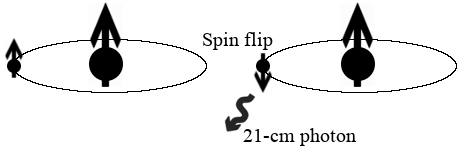
\includegraphics[width=0.55\textwidth]{spin_flip.png}
	\caption[The spin-flip transition of neutral hydrogen]{An illustration of the spin-flip transition of neutral hydrogen. Initially, the spin of the electron is parallel with that of the proton---both are in a ``spin up'' state. This initial state is at a higher energy than when the spin of the electron and proton are antiparallel. The transition occurs when the spin of the electron flips from up to down, emitting a photon with a wavelength of 21 cm.}
	\label{fig:spin_flip}
\end{figure}

\tocless\subsection{\hypertarget{subsec:rfi}{1.5.\hspace{0.75em}Radio Frequency Interference}}
\addcontentsline{toc}{subsection}{1.5.\hspace{0.75em}Radio Frequency Interference}

Interference from sources such as FM radio, satellite and aircraft communications, and television transmissions is exceptionally bright and can easily contaminate the results of any cosmological measurement. Unfortunately, since it is typically man-made, it is also everywhere that humans are.

There are a few ways to mitigate RFI. First, instruments can be built in remote areas to minimize contact with human-made interference. Then, after taking observations, RFI can be removed with software that detects and masks out (``flags'') data it identifies as being contaminated. Steps further along in the data reduction and analysis process ignore this flagged data.

There are currently several radio interferometers making observations towards a 21-cm power spectral EoR detection, some of which are located in remote places of the world and all of which use some sort of RFI excision software. The Hydrogen Epoch of Reionization Array (HERA), currently under construction in the Karoo Desert in South Africa, does both. \vspace{3mm}

\tocless\subsection{\hypertarget{subsec:hera}{1.6.\hspace{0.75em}The Hydrogen Epoch of Reionization Array}}
\addcontentsline{toc}{subsection}{1.6.\hspace{0.75em}The Hydrogen Epoch of Reionization Array}

\begin{figure}[tb]
	\centering
	\begin{subfigure}{0.48\textwidth}
		\centering
		{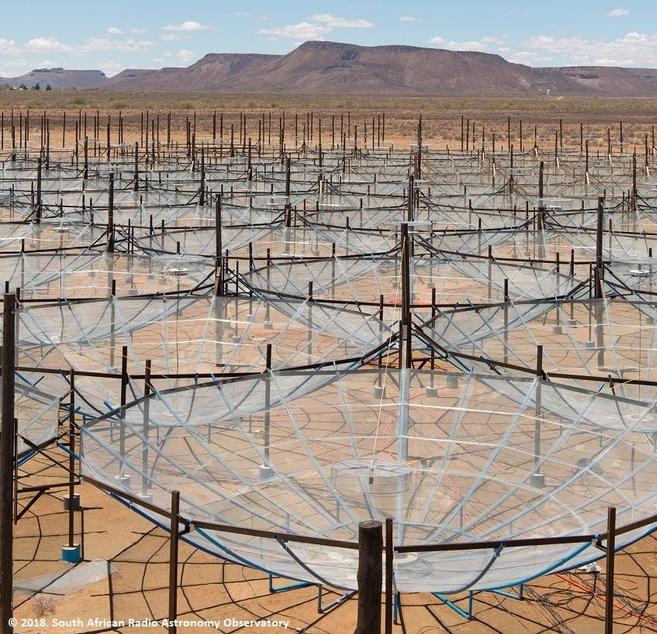
\includegraphics[width=\textwidth]{hera.png}}
	\end{subfigure} \hfill
	\begin{subfigure}{0.48\textwidth}
		\centering
		{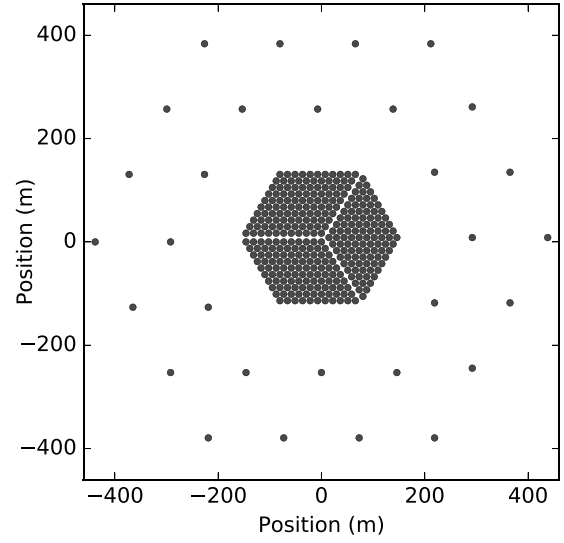
\includegraphics[width=\textwidth]{hera_map.png}}
	\end{subfigure}
	\caption[The Hydrogen Epoch of Reionization Array]{Left: A photo of HERA as of late 2017 -- early 2018. HERA will observe the periods prior to and during the EoR via the redshifted 21-cm line from the IGM. Image courtesy of the South African Radio Astronomy Observatory. Right: A map of the completed array, composed of 320 central elements and 30 outriggers \citep{deboer2017}.}
	\label{fig:hera}
\end{figure}

HERA (Figure \ref{fig:hera}) is one of several radio interferometers designed to study the large-scale structure during the EoR via power spectral measurements of the redshifted 21-cm line \citep{deboer2017}---others include the Low Frequency Array \citep[LOFAR;][]{vanHaarlem2013} and the Murchison Widefield Array \citep[MWA;][]{tingay2013}. HERA builds upon preceding instruments, such as the MWA and the Donald C. Backer Precision Array for Probing the Epoch of Reionization \citep[PAPER;][]{parsons2010}, and will pave the way for future experiments such as the Square Kilometer Array \cite[SKA; e.g.,][]{mellema2013}. HERA specifically uses the so-called ``delay spectrum'' approach introduced in \cite{parsons2012}, which attempts to maximize sensitivity in the desired modes while rejecting modes contaminated by foreground power, to make this measurement.

When complete, HERA will be composed of 350 14-meter dishes with a tightly-packed 320-element hexagonal core and 30 outriggers (right panel of Figure \ref{fig:hera}). The dense arrangement was chosen to maximize sensitivity to the diffuseness of the 21-cm signal, which will be sampled primarily by short baselines. The hexagonal shape creates redundancies in Fourier space (baselines oriented in the same direction, no matter their physical location, will be sensitive to the same Fourier modes of the sky), which increases sensitivity and the efficacy of the delay spectrum approach for separating and rejecting foreground-contaminated modes and allows for the redundant calibration technique developed and pioneered in \cite{liu2010} and \cite{zheng2014}.

HERA's first scientific observing campaign took place from September 2017 to the beginning of April 2018, with the first fully processed internal data release, H1C (HERA with $\sim 100$ antennas) IDR 2.1, occurring in June 2018 (public HERA memo \href{http://reionization.org/wp-content/uploads/2018/07/IDR2.1_Memo_v2.html}{\#45}). A broad overview of the data processing can be found in section 5 in the same memo, but key steps to note are several calibration steps (e.g., redundant calibration and absolute gain calibration) and RFI flagging. \vspace{3mm}

\tocless\section{\hypertarget{sec:rfipspec}{2.\hspace{0.75em}RFI and the Power Spectrum}}
\addcontentsline{toc}{section}{2.\hspace{0.75em}RFI and the Power Spectrum}

All data products used were from H1C IDR 2.1. These observations were already calibrated, RFI-flagged, and otherwise reduced in a collaboration pipeline, although a summary of important steps follows. \vspace{3mm}

\tocless\subsection{\hypertarget{subsec:h1crfi}{2.1.\hspace{0.75em}H1C IDR 2.1 RFI Excision}}
\addcontentsline{toc}{subsection}{2.1.\hspace{0.75em}H1C IDR 2.1 RFI Excision}

\begin{figure}[p]
	\centering
	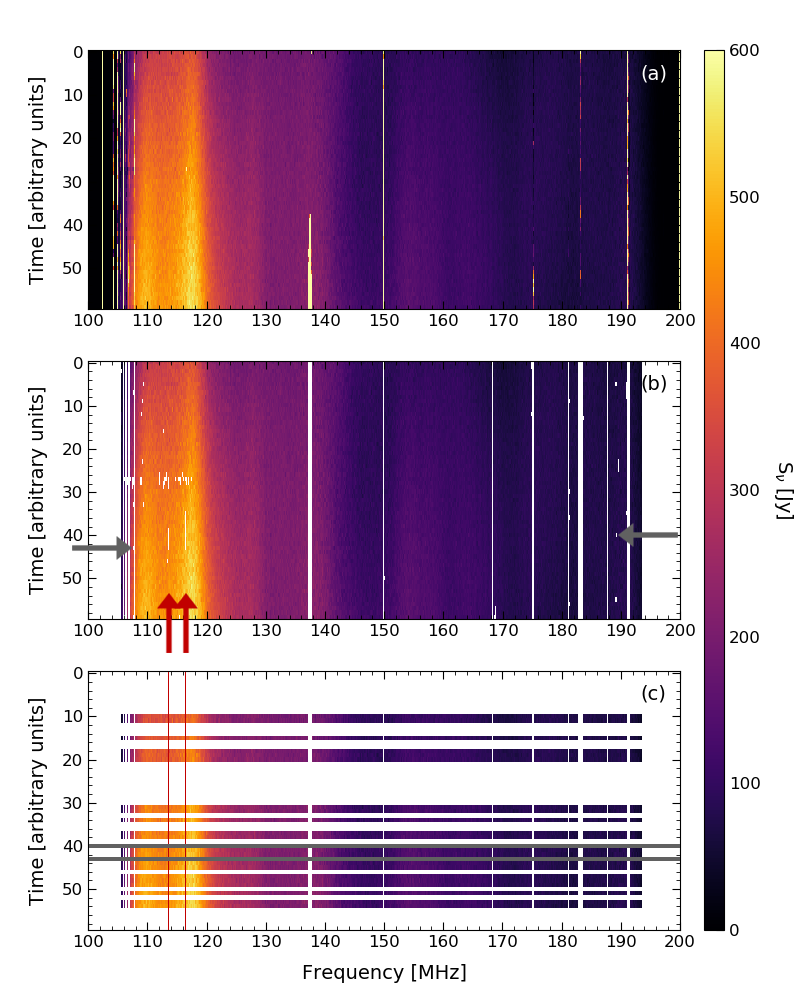
\includegraphics[width=\textwidth]{flagging_steps_arrows.png}
	\caption[Steps for flagging RFI]{An example of the process of flagging RFI from (a) unflagged visibilities to (b) XRFI flags, and finally (c) broadcasted flags. The red arrows in (b) indicate frequency pixels with enough flags to flag the entire channel as determined by the procedure described in Section \hyperlink{subsec:h1crfi}{2.1}, with the flagged channels shown by the red lines in (c). Similarly, grey arrows and lines indicate the initial flags and subsequent broadcasting for time integrations that were completely flagged.}
	\label{fig:rfi_flagging}
\end{figure}

The H1C IDR 2.1 data reduction pipeline utilized code developed for HERA quality assurance (\heraqm\footnote{\url{https://github.com/HERA-team/hera_qm}}) to identify and flag RFI. The entire flagging pipeline, XRFI, functioned as follows:

\begin{enumerate}
	\item Data for individual antennas or baseline were detrended with a median filter by calculating the difference between the data and median and dividing by the noise.
	\item The same data were flagged based on user-defined thresholds.
	\item Flags from individual antennas/baselines were averaged over time, thresholded, and flagged again over a full file.
	\item The data were delay filtered to remove foregrounds.
	\item Visibilities were flagged following the procedure in steps 1 -- 3 and combined into final observation flags.
\end{enumerate}

This process is generally relatively intuitive when the data are examined by eye in the time-frequency domain as in Figure \ref{fig:rfi_flagging}. Panel (a) is the original, unflagged data with yellow stripes and pixels where interference is present. Panel (b) shows the mask determined by XRFI, where white pixels denote flagging. These approximately correspond to RFI that can be seen by eye in panel (a), although not perfectly. \vspace{3mm}

\tocless\subsection{\hypertarget{subsec:pspecestimation}{2.2.\hspace{0.75em}Estimating the Power Spectrum}}
\addcontentsline{toc}{subsection}{2.2.\hspace{0.75em}Estimating the Power Spectrum}

The 21-cm power spectrum $P_{21}\left(\vec{k}\right)$ is mathematically defined as
\begin{equation}
\left\langle \widetilde{T}_b\left(\vec{k}\right) \widetilde{T}_b^*\left(\vec{k'}\right) \right\rangle = \left(2\pi\right)^3 \delta\left(\vec{k} - \vec{k'}\right) P_{21}\left(\vec{k}\right)
\label{eqn:P21}
\end{equation}
where $\widetilde{T}_b\left(\vec{k}\right)$ is the 3D spatial Fourier transform of the brightness temperature distribution on the sky and $\delta$ is the Dirac delta function. Note that Equation \ref{eqn:P21} contains two continuous functions, $T_b$ and $P_{21}$, which must be discretized to be computationally feasible.

To perform this discretization, the HERA collaboration's power spectrum estimation code, \herapspec\footnote{\url{https://github.com/HERA-team/hera_pspec}}, uses an optimal quadratic estimator---the same approach was used for PAPER analysis \citep{ali2015}, with further information in, e.g., \cite{tegmark1997}, \cite{tegmark1998}, and \cite{liu2011}. A particular quirk of the HERA power spectrum estimation implementation requires that interference flagging is time-independent. That is, the flagging pattern for any given time in an observation is the same as that of all other times in that observation. This is to allow for the same statistical assumptions to be made for all times and is faster and simpler than recalculating statistics for every time integration used to estimate a power spectrum, although time-dependent approaches are a future goal.

To satisfy this requirement, after flagging with XRFI, the flags are broadcast such that the patterns are time-independent for a fixed baseline and spectral window. For a given frequency pixel (also called a channel) in the selected spectral window, if the total fraction of flagged times in that channel exceeds a user-defined threshold, then the entire channel is flagged. Otherwise, if the flagged times in the channel do not exceed the threshold, any time integrations that contain flags are flagged for all frequencies in the spectral window. This process is carried out for each frequency pixel until all flags are time independent. Panel (c) of Figure \ref{fig:rfi_flagging} shows an example of this broadcasting in practice. Recall that the broadcasting is not part of the standard data processing pipeline, but is a specific requirement of using \herapspec~to estimate a power spectrum. \vspace{3mm}

\tocless\subsection{\hypertarget{subsec:refpspec}{2.3.\hspace{0.75em}Reference Power Spectrum}}
\addcontentsline{toc}{subsection}{2.3.\hspace{0.75em}Reference Power Spectrum}

Using the methods outlined in Sections \hyperlink{subsec:h1crfi}{2.1} and \hyperlink{subsec:pspecestimation}{2.2}, I used real HERA data to test the effects of various RFI removal strategies on the power spectrum. I first constructed a ``control'' spectrum using a 100-channel (approximately 10 MHz) band uncontaminated by RFI, I calculated this ``ground truth'' power spectrum without any flags (Figure \ref{fig:noflags}). The innermost $\sim 1 \; k_\parallel$ are dominated by power from galactic and extragalactic radio foregrounds, so for the remainder of this work, we will focus on the effects at larger values of $k_\parallel$ outside the central peak.

\begin{figure}[p]
	\centering
	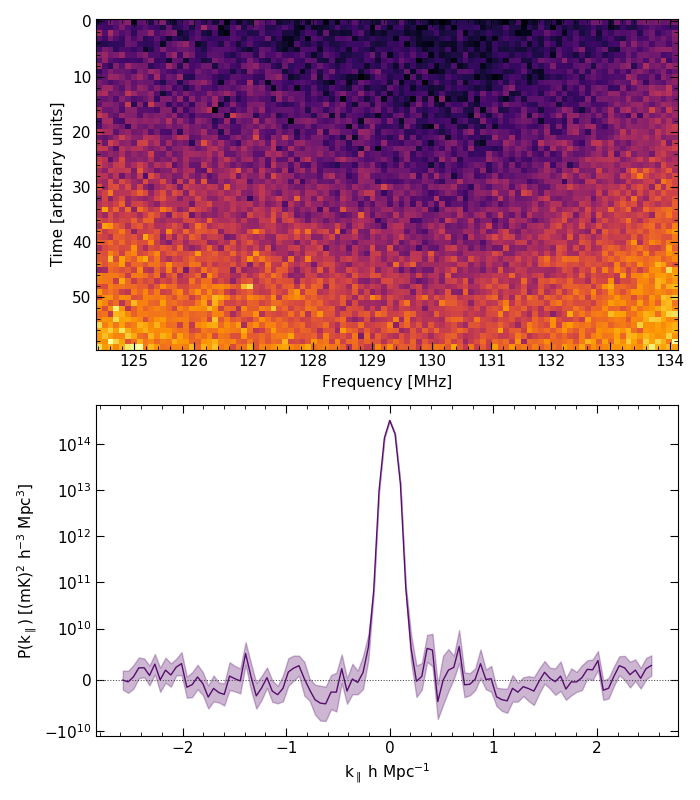
\includegraphics[width=\textwidth]{42378_noflags.png}
	\caption[Original power spectrum]{Power spectrum estimated with unflagged real data (top panel) over an approximately 9.75 MHz frequency range. The central peak is due to power from foregrounds, so we expect to measure the EoR in the wings where this power spectrum fluctuates close to zero.}
	\label{fig:noflags}
\end{figure}

\begin{figure}[p]
	\centering
	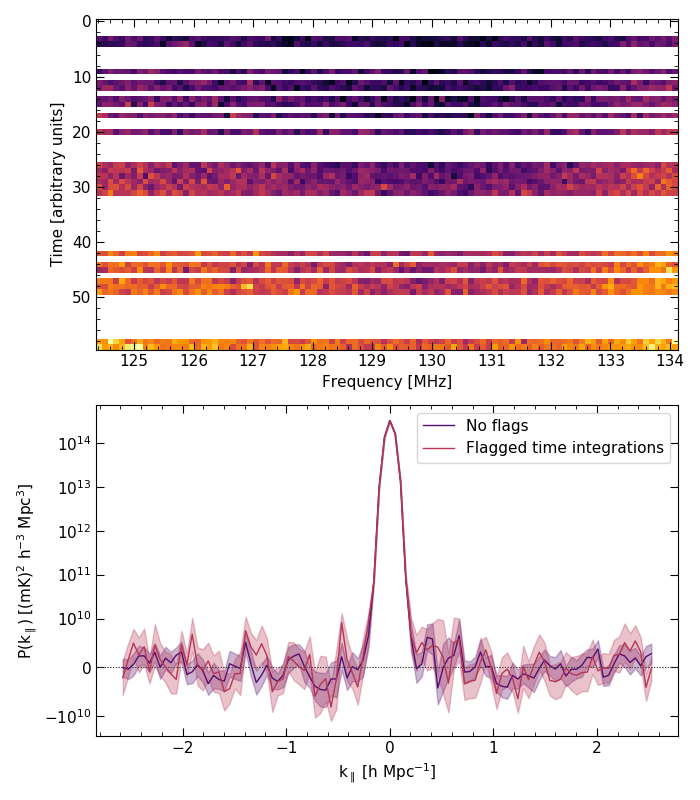
\includegraphics[width=\textwidth]{42378_timeflags.png}
	\caption[Power spectrum calculated with data flagged only in time]{Comparison of the control spectrum and the spectrum estimated with data flagged as in the top panel, which only has broadband flags. There are no obvious systematic effects, and the two spectra are generally consistent with each other and with zero within errors.}
	\label{fig:time_flags}
\end{figure}

The single spectrum in Figure \ref{fig:noflags} was calculated by estimating individual spectra for all combinations of cross multiples of baselines in a redundant group (14-m east-west baselines) and taking the average, with errors from bootstrapping over baseline pair cross multiples. \note{[LW: This is kind of opaque wording, am open to suggestions.]} In practice, the data that will be used for HERA power spectrum analyses, at least regarding interference, will likely be similar to that in Figure \ref{fig:noflags}---uncontaminated and unflagged. However, for our purposes, we would like to investigate the effects of different RFI flagging strategies.

These flags take two forms: flags over the full band for a few time integrations, or narrowband flags for all times. Figure \ref{fig:time_flags} shows a comparison of a power spectrum estimated with data flagged over the entire band for specific time integrations. If there are any systematic effects introduced by this flagging, they are not extremely overt, although more subtle ones may be masked by noise and other observational uncertainties. \vspace{3mm}

\tocless\subsection{\hypertarget{subsec:narrowband}{2.4.\hspace{0.75em}Narrowband Flagging}}
\addcontentsline{toc}{subsection}{2.4.\hspace{0.75em}Narrowband Flagging}

\begin{figure}[p]
	\centering
	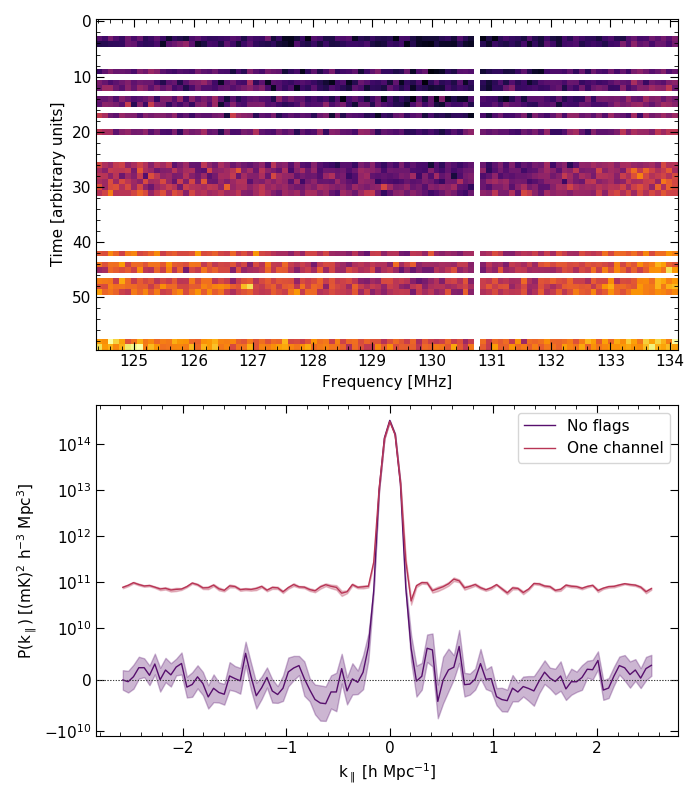
\includegraphics[width=\textwidth]{42378_flag315.png}
	\caption[Power spectrum calculated with flagged time integrations and one flagged channel]{The power spectrum after flagging one frequency channel.}
	\label{fig:flag_chan315}
\end{figure}

\begin{figure}[p]
	\centering
	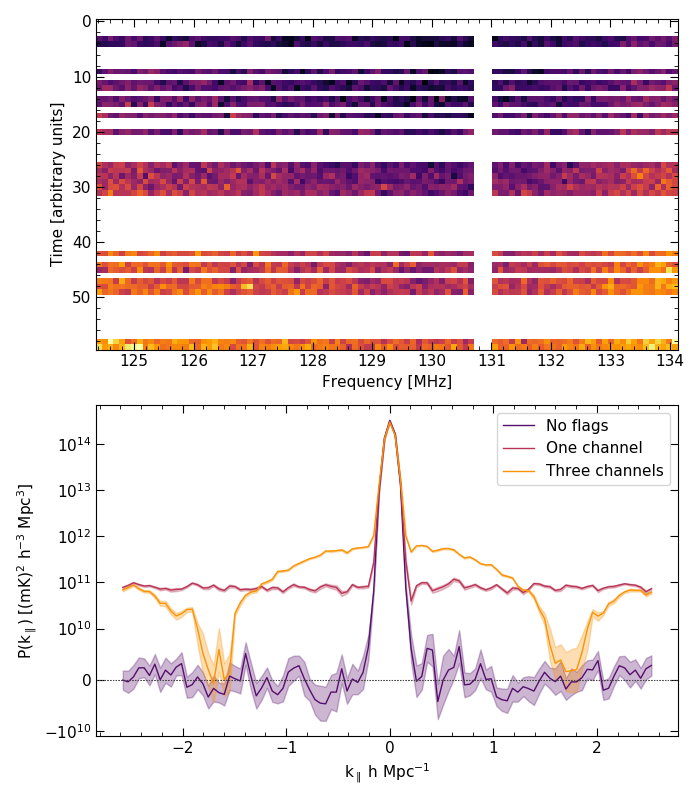
\includegraphics[width=\textwidth]{42378_flag315_317.png}
	\caption[Power spectrum calculated with flagged time integrations and three contiguous flagged channels]{The power spectrum estimated after flagging a contiguous block of three channels.}
	\label{fig:flag_chan315_317}
\end{figure}

\begin{figure}[p]
	\centering
	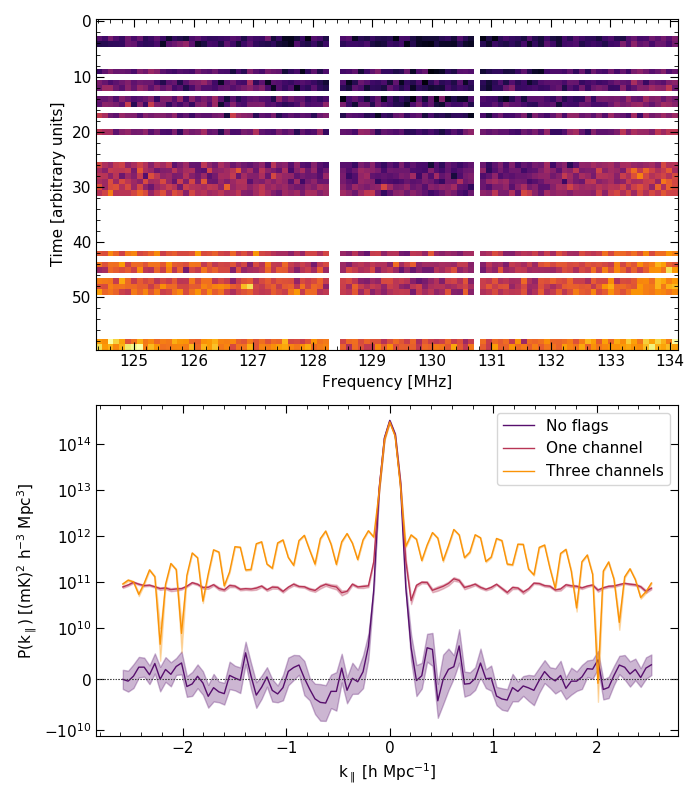
\includegraphics[width=\textwidth]{42378_flag290_291_315.png}
	\caption[Power spectrum calculated with flagged time integrations and three flagged channels (two contiguous, one not)]{The power spectrum after flagging two adjacent channels and one non-adjacent channel.}
	\label{fig:flag_chan290_291_315}
\end{figure}

We also test the effects of the other flagging pattern present: narrowband flags for all times. A number of parameters for these flags can vary, and we focus on examining the number of consecutively flagged frequency pixels and the relative location of the flags within the spectral window of interest. We test a variety of flags exploring a few features of different combinations of locations and multiple flags in the frequency range, but it should be noted that the experiments we ran do not span the parameter space of flagging patterns.

The most basic experiment is to inject a single flagged channel. Figure \ref{fig:flag_chan315} shows the resulting flagging pattern and the power spectrum. With the flag approximately 15 channels away from the center of the band, the outer wings of the power spectrum are approximately consistent with $10^{11}$, eleven orders of magnitude higher in the wings than the original unflagged spectrum. Moving the flag further from the center by another ten channels lowers this by about a dex, and when the flag is 15 channels from the edge, the spectrum is again consistent with zero. This is likely due to the spectral tapering function: the closer to the edge, the more the data are down-weighted by the tapering. Thus, the contribution of the edge data, or lack thereof, is smaller.

As another test, we also flag progressively more channels in a continuous block near our first narrowband flag. Figure \ref{fig:flag_chan315_317} compares the result after flagging three contiguous channels to both the unflagged spectrum and the spectrum after flagging only one channel. Examples with two and four flagged channels are in the \hyperlink{appendix}{Appendix}. While this spectrum is, like the single-channel-flagged spectrum, also at a systematically higher level than the unflagged spectrum for most values of $k_\parallel$, it also exhibits significant periodic structure. The exact number of ``cycles'' in the power spectrum increases with increasing number of flagged channels, and as the flagged channels are moved closer to the edge of the spectral window, the minimum of the spectrum increases towards $\sim 10^{11}$.

The final test we run on the real data is flagging non-contiguous frequency pixels. Figure \ref{fig:flag_chan290_291_315} shows an example spectrum from flagging two adjacent channels and one isolated channel. Again, variations on this approach are in the \hyperlink{appendix}{Appendix}. It appears that the fast fluctuations arise from the gaps in frequency of the flags and the larger-scale taper mimics the behavior of the spectrum in Figure \ref{fig:flag_chan315_317} (or more comparably, Figure \ref{fig:flag_chan315_316} in the \hyperlink{appendix}{Appendix}). That is, it appears that more than one flagged channel introduces the taper, while having more than one flag separated in frequency in the spectral window contributes small-scale oscillations Of the experiments we ran, this one reached the highest values outside the central peak, and also shows the most spectral structure. As was the case previously, the location of the flags in the spectral window plays a significant role on how the final power spectrum is impacted; as the flags approach the edges, the spectra approach the unflagged result. \vspace{3mm}

\begin{figure}[t]
	\centering
	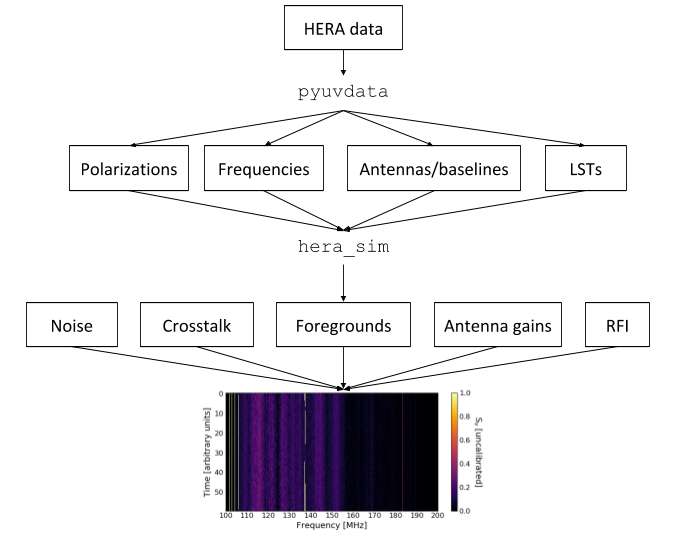
\includegraphics[width=\textwidth]{sim_flow.png}
	\caption[Flowchart of the process of modelling HERA data]{A flowchart of the process used to simulate HERA data. In particular, the foreground model is based off of parameters from real data. RFI, noise, antenna gains, and crosstalk (when the signal from two antennas gets erroneously correlated) calculated independently by \herasim~are added to yield a mock dataset.}
	\label{fig:sim_flow}
\end{figure}

\tocless\section{\hypertarget{sec:modelling}{3.\hspace{0.75em}Modelling HERA Data}}
\addcontentsline{toc}{section}{3.\hspace{0.75em}Modelling HERA Data}

\begin{figure}[p]
	\centering
	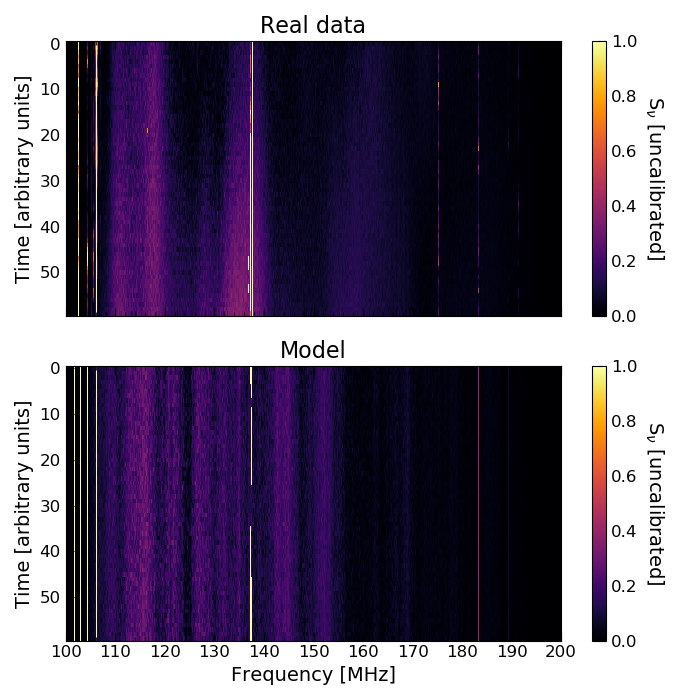
\includegraphics[width=\textwidth]{sim_comparison.png}
	\caption[Comparison of simulated and real data]{A comparison between the model data and the real data used to obtain parameters for the simulation for one 14-meter baseline. Particular interference features to note include the Orbcomm satellite constellation downlink at approximately $137$ MHz, broadcasts from FM radio at lower frequencies, and TV transmissions at higher frequencies.}
	\label{fig:sim_comparison}
\end{figure}

In order to perform experiments in a more controlled setting, I modelled HERA data with the simple visibility simulator \herasim\footnote{\url{https://github.com/HERA-team/hera_sim}}. Using the package \pyuvdata\footnote{\url{https://github.com/RadioAstronomySoftwareGroup/pyuvdata}} as an interface between HERA data files and \herasim, I used real observation parameters such as observed frequencies, local sidereal times (LSTs), antenna positions, baselines, and polarizations as inputs to the simulator. This was done in an effort to create realistic realizations of what HERA might actually observe. Figure \ref{fig:sim_flow} is a flow chart of this process and Figure \ref{fig:sim_comparison} shows an example of the resulting model and the uncalibrated real data scaled to match the model.

Since RFI is the focus of this work, I took care to roughly match the RFI patterns in the simulation to those present in real data. In particular, I focused on matching three interference features: the Orbcomm satellite constellation downlink at $137 - 138$ MHz, FM radio broadcasts at frequencies less than $108$ MHz, and the occasional VHF TV transmission above $\sim 175$ MHz. All of these can be seen as thin vertical lines in Figure \ref{fig:sim_comparison}.

\tocless\subsection{\hypertarget{subsec:simtests}{3.1.\hspace{0.75em}Model Power Spectra}}
\addcontentsline{toc}{subsection}{3.1.\hspace{0.75em}Model Power Spectra}

\begin{figure}[t]
	\centering
	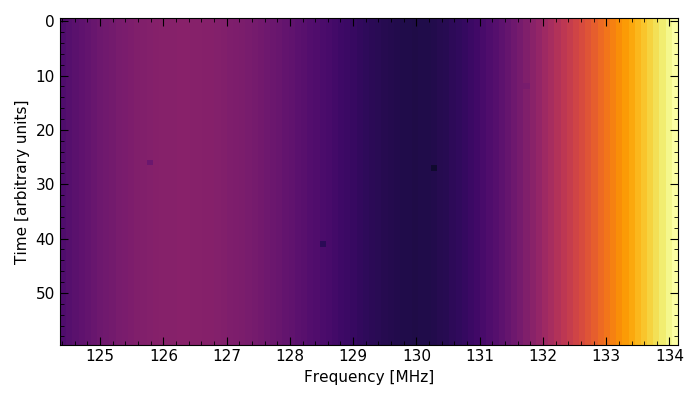
\includegraphics[width=\textwidth]{49088_sim_data.png}
	\caption[Model data]{Simulated HERA foregrounds based on parameters from observations.}
	\label{fig:sim_data}
\end{figure}

I was particularly interested in the effect of broadband flags for select time integrations. In Figure \ref{fig:time_flags}, it was difficult to see any systematic changes in the power spectrum, if there were any, due to the fluctuations in the spectrum. Thus, for the express purpose of studying this, we only modelled foregrounds (Figure \ref{fig:sim_data}). This also allowed us to more clearly see the effects of flags without instrumental effects as are present in the real data. In particular, there is also no RFI; instead, we copied the broadcasted flags from a real observation and applied them to the model data.

Figure \ref{fig:sim_time_flags} compares the unflagged and time-integration-flagged power spectra. The difference between them is nearly nonexistent (the flagged power spectrum is $< 1.5$ times the unflagged one in the wings), confirming our initial impression from the real data that flagging only time integrations has very little effect on the power spectrum.

\begin{figure}[p]
	\centering
	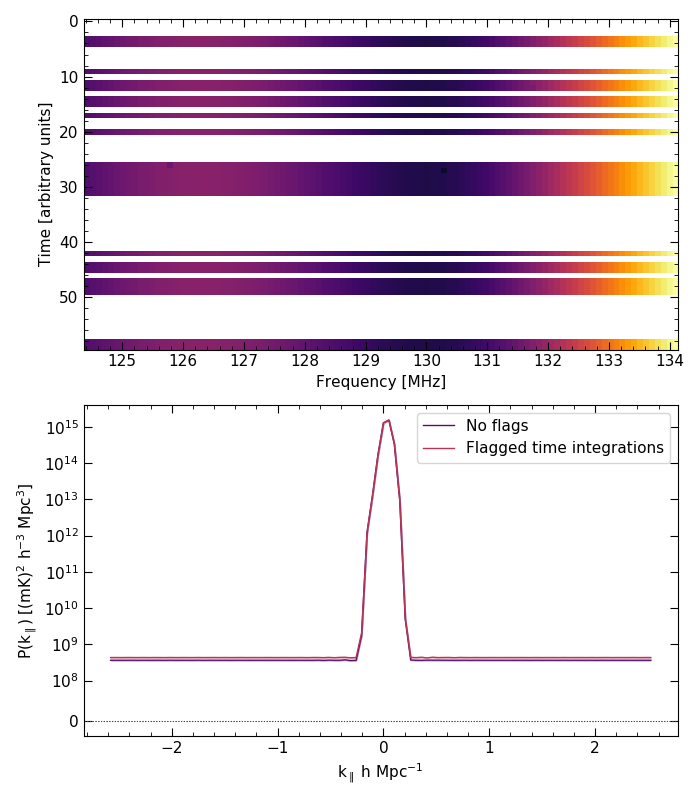
\includegraphics[width=\textwidth]{49088_sim_timeflags.png}
	\caption[Model power spectrum calculated with data flagged only in time]{Comparison of original, unflagged model power spectrum and the model power spectrum calculated with broadband flags.}
	\label{fig:sim_time_flags}
\end{figure}

\begin{figure}[p]
	\centering
	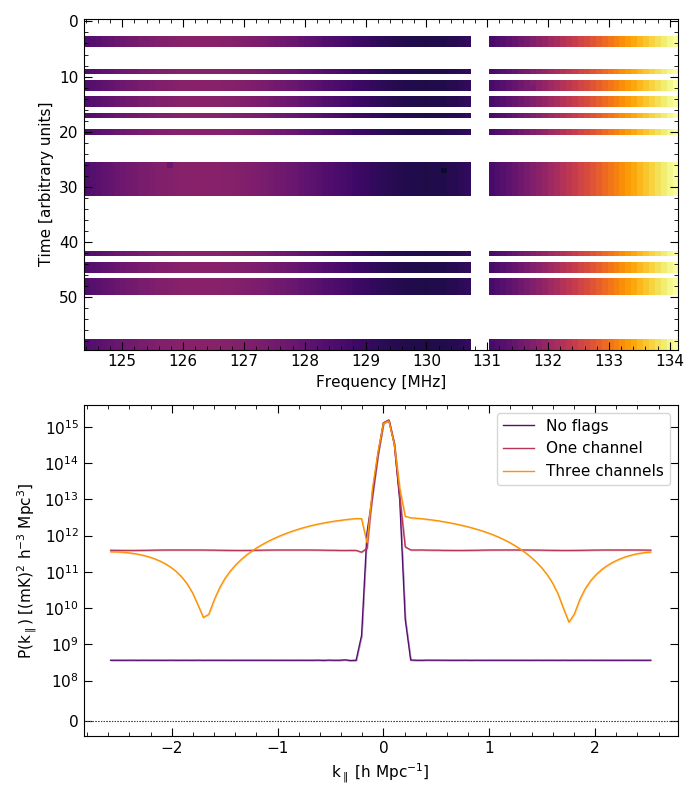
\includegraphics[width=\textwidth]{49088_sim_flag315_317.png}
	\caption[Model power spectrum calculated with flagged time integrations and three contiguous flagged channels]{Simulated power spectrum calculated with three contiguous flagged channels.}
	\label{fig:sim_flag_chan315_317}
\end{figure}

We continue by recreating the tests we ran on the real data, and find broad qualitative agreement (e.g., Figure \ref{fig:sim_flag_chan315_317} corresponds with Figure \ref{fig:flag_chan315_317}; remaining spectra are in the \hyperlink{appendix}{Appendix}). Quantitative comparison is difficult at this point in time since the unflagged power spectrum is not consistent with zero outside the central peak, which merits further refinement in the future, especially for the purposes of drawing numerical conclusions. \vspace{3mm}

\tocless\section{\hypertarget{sec:conclusion}{4.\hspace{0.75em}Conclusion}}
\addcontentsline{toc}{section}{4.\hspace{0.75em}Conclusion}

The Epoch of Reionization is still one of the most mysterious periods in our universe's history. Filling in the story of cosmic evolution with the timeline and topography of the EoR will provide the beginnings of a much-needed bridge between the CMB and the rich structure we see today. Measuring and analyzing the power spectrum of the 21-cm with HERA, among other current and next-generation instruments, will be a key component of building that bridge.

Several challenges, not the least of which are bright radio foregrounds, stand between us and studying the EoR with this method. However, though radio foregrounds are the largest obstacle, even a single misunderstood or uncorrected systematic error makes a detection more difficult. Such systematics can range from instrumental effects that aren't quite calibrated correctly to man-made interference.

Towards the goal of making this detection, I have focused on characterizing the effects of RFI on the power spectrum. In particular, I have used methods and techniques already developed by the HERA collaboration in an attempt to recreate the circumstances under which future analyses will be undertaken. This includes everything from initial RFI identification and flagging to the final estimation of the power spectrum.

In the future, we would like to quantify the effects seen qualitatively in this work. In particular, we will place a special emphasis on statistically describing the differences in the power spectra arising from different flagging strategies and patterns. Once we have reached a more complete understanding of existing RFI mitigation approaches and their impacts on the final cosmological result, we will place an approximate limit on how effective our removal strategy will need to be to detect the EoR. Then, we will be able to develop improved RFI excision algorithms and other strategies to minimize the effects of RFI flagging and incorporate them into the HERA data processing and power spectrum pipelines. \vspace{3mm}

\tocless\section{\hypertarget{references}{References}}
\addcontentsline{toc}{section}{References}
\bibliographystyle{aasjournal}
\bibliography{refs}

\newpage
\tocless\section{\hypertarget{appendix}{Appendix}}
\addcontentsline{toc}{section}{Appendix}

Here, we include additional experiments testing different flagging patterns and the resulting 21-cm power spectrum.

\begin{figure}[th]
	\centering
	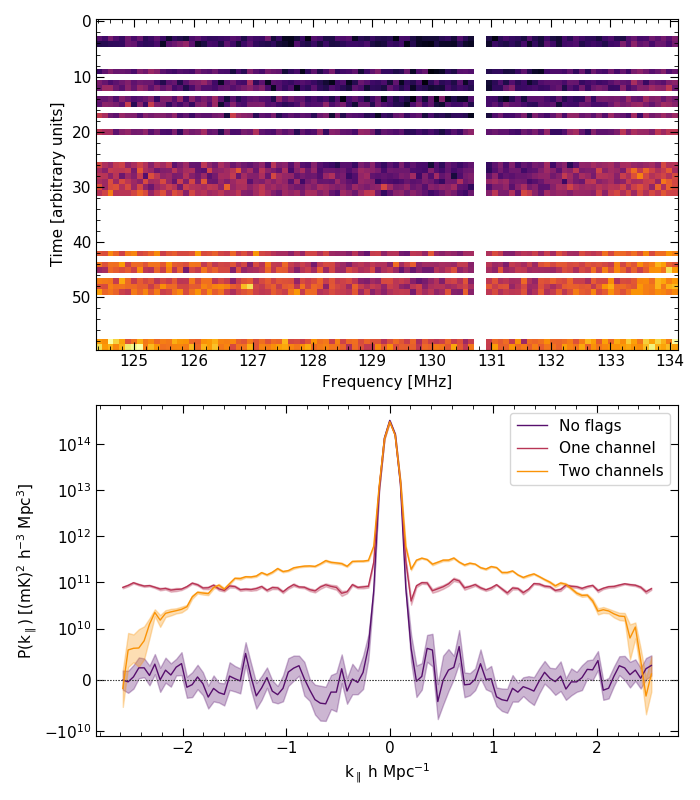
\includegraphics[width=0.95\textwidth]{42378_flag315_316.png}
	\caption[Power spectrum calculated with flagged time integrations and two contiguous flagged channels]{The power spectrum estimated after flagging a contiguous block of two channels.}
	\label{fig:flag_chan315_316}
\end{figure}

\begin{figure}[p]
	\centering
	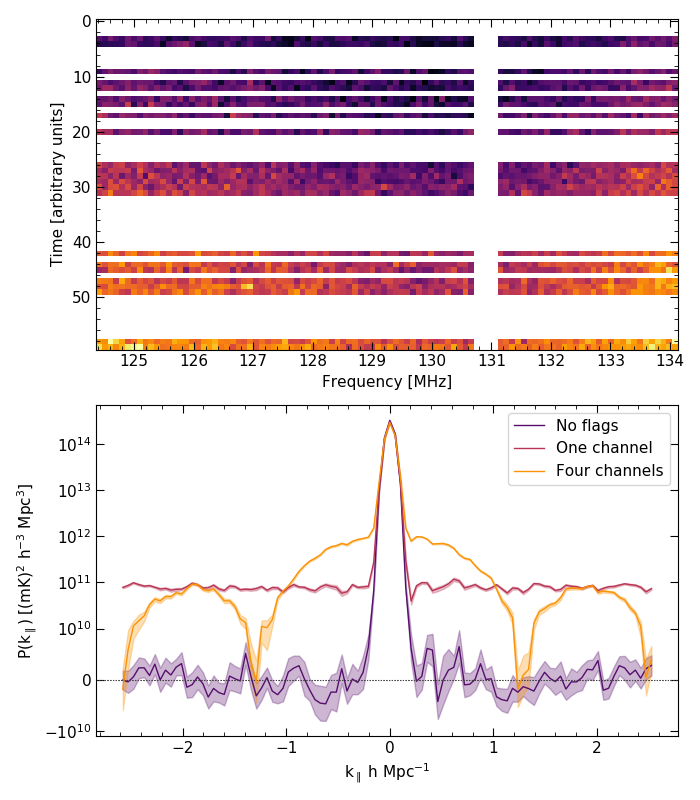
\includegraphics[width=0.95\textwidth]{42378_flag315_318.png}
	\caption[Power spectrum calculated with flagged time integrations and four contiguous flagged channels]{The power spectrum estimated after flagging a contiguous block of four channels.}
	\label{fig:flag_chan315_318}
\end{figure}

\begin{figure}[p]
	\centering
	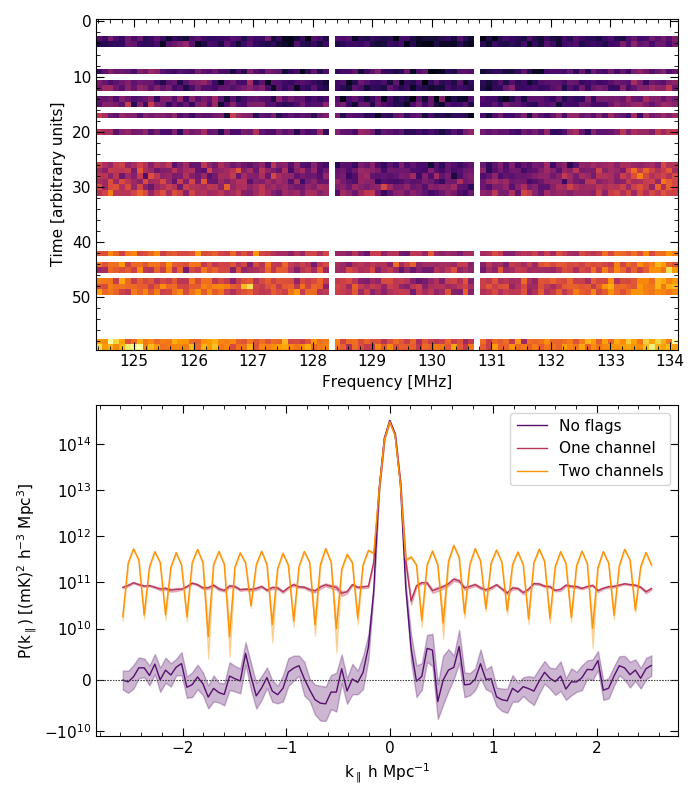
\includegraphics[width=0.95\textwidth]{42378_flag290_315.png}
	\caption[Power spectrum calculated with flagged time integrations and two non-contiguous flagged channels]{The power spectrum estimated after flagging two channels separated in frequency.}
	\label{fig:flag_chan290_315}
\end{figure}

\begin{figure}[p]
	\centering
	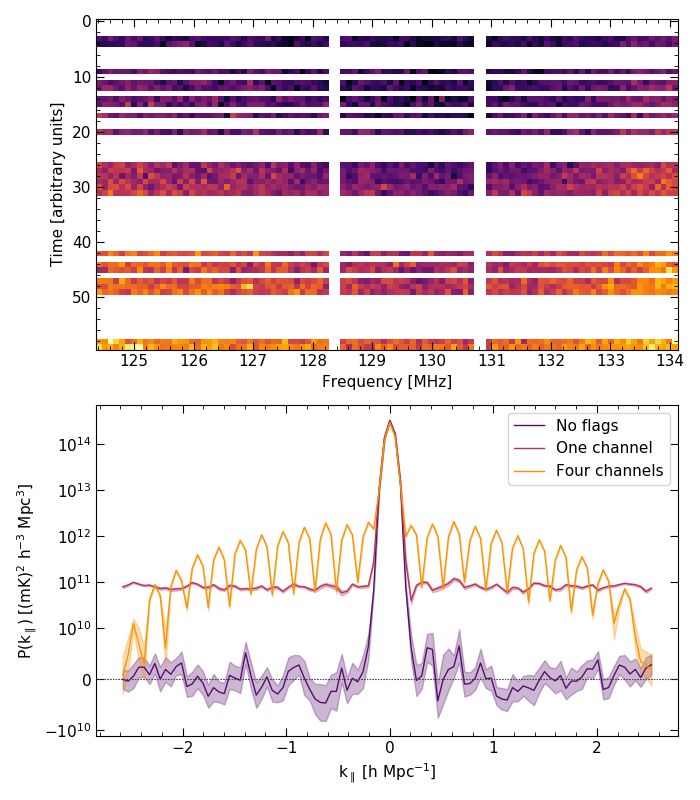
\includegraphics[width=0.95\textwidth]{42378_flag290_291_315_316.png}
	\caption[Power spectrum calculated with flagged time integrations and four flagged channels (two blocks of two channels)]{Caption}
	\label{fig:flag_chan290_291_315_316}
\end{figure}

\begin{figure}[p]
	\centering
	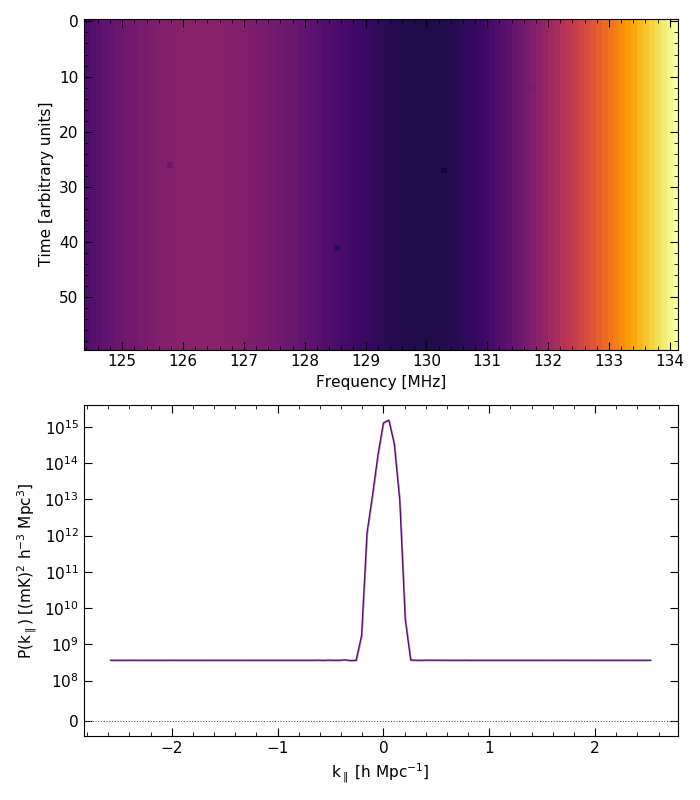
\includegraphics[width=0.95\textwidth]{49088_sim_noflags.png}
	\caption[Original model power spectrum (only foregrounds)]{Power spectrum calculated with unflagged model data.}
	\label{fig:sim_noflags}
\end{figure}

\begin{figure}[p]
	\centering
	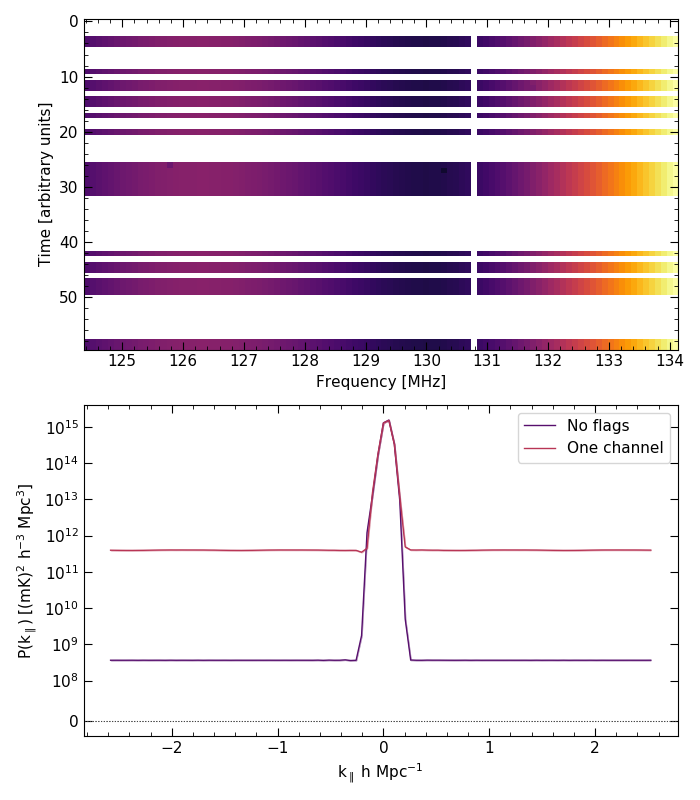
\includegraphics[width=0.95\textwidth]{49088_sim_flag315.png}
	\caption[Model power spectrum calculated with flagged time integrations and one flagged channel]{Simulated power spectrum calculated with one flagged channel.}
	\label{fig:sim_flag_chan315}
\end{figure}

\begin{figure}[p]
	\centering
	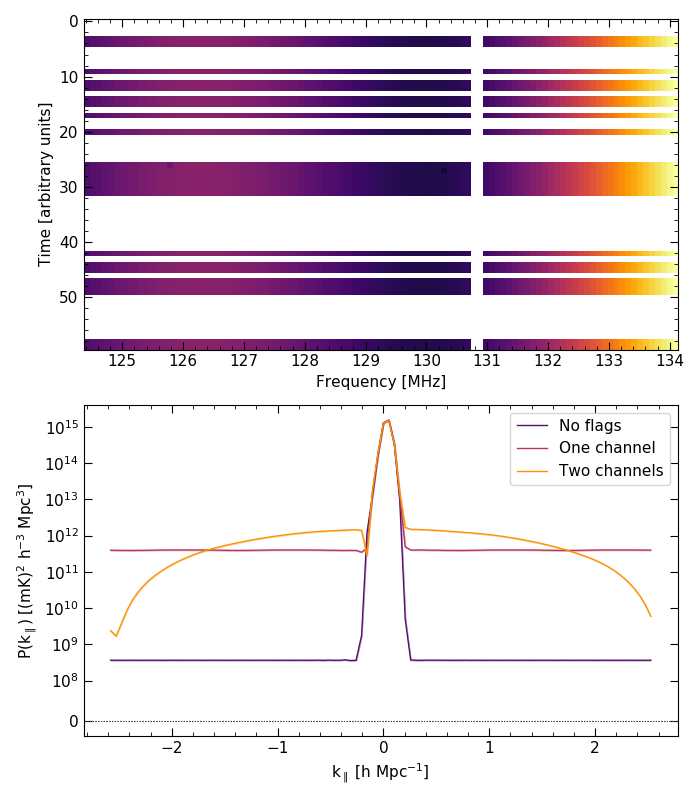
\includegraphics[width=\textwidth]{49088_sim_flag315_316.png}
	\caption[Model power spectrum calculated with flagged time integrations and two contiguous flagged channels]{Simulated power spectrum calculated with two contiguous flagged channels.}
	\label{fig:sim_flag_chan315_316}
\end{figure}

\begin{figure}[p]
	\centering
	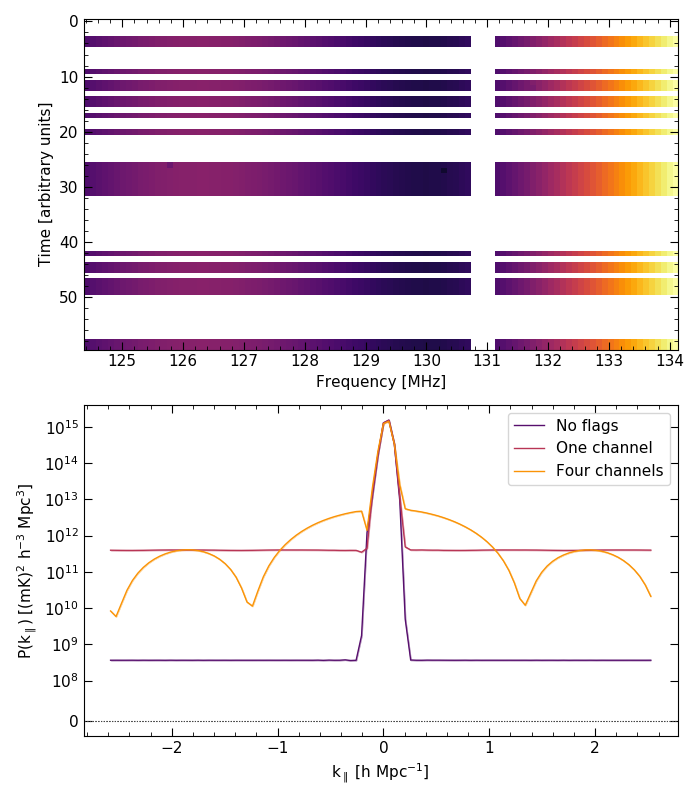
\includegraphics[width=\textwidth]{49088_sim_flag315_318.png}
	\caption[Model power spectrum calculated with flagged time integrations and four contiguous flagged channels]{Simulated power spectrum calculated with four contiguous flagged channels.}
	\label{fig:sim_flag_chan315_318}
\end{figure}

\begin{figure}[p]
	\centering
	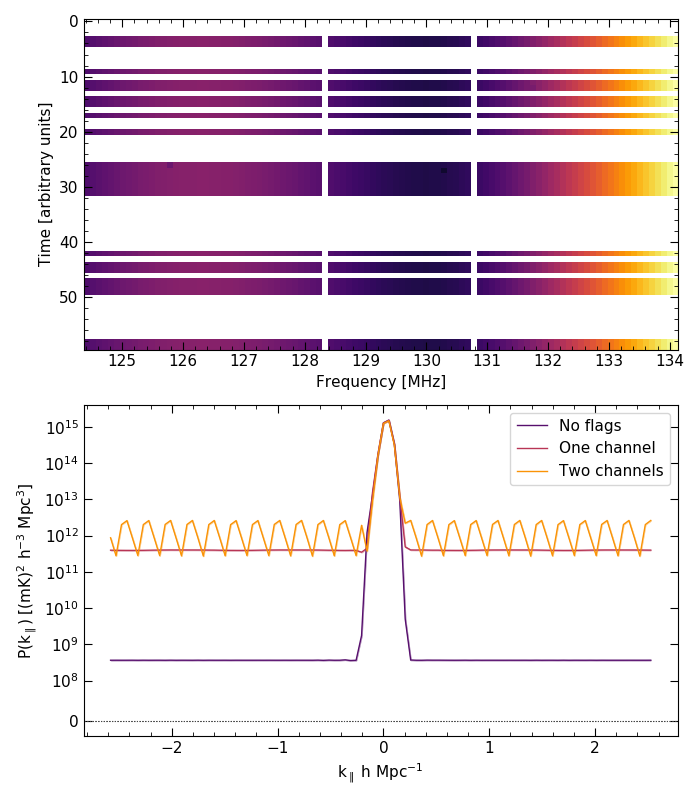
\includegraphics[width=\textwidth]{49088_sim_flag290_315.png}
	\caption[Model power spectrum calculated with flagged time integrations and two non-contiguous flagged channels]{Simulated power spectrum calculated with two non-contiguous flagged channels.}
	\label{fig:sim_flag_chan290_315}
\end{figure}

\begin{figure}[p]
	\centering
	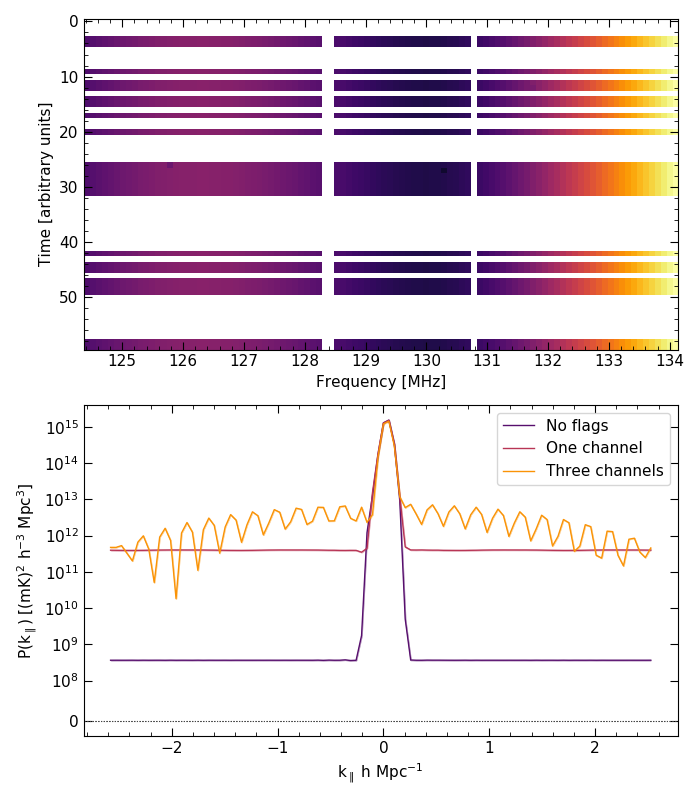
\includegraphics[width=\textwidth]{49088_sim_flag290_291_315.png}
	\caption[Model power spectrum calculated with flagged time integrations and three flagged channels (two contiguous, one not)]{Simulated power spectrum calculated with three flagged channels, two adjacent and one not.}
	\label{fig:sim_flag_chan290_291_315}
\end{figure}

\begin{figure}[p]
	\centering
	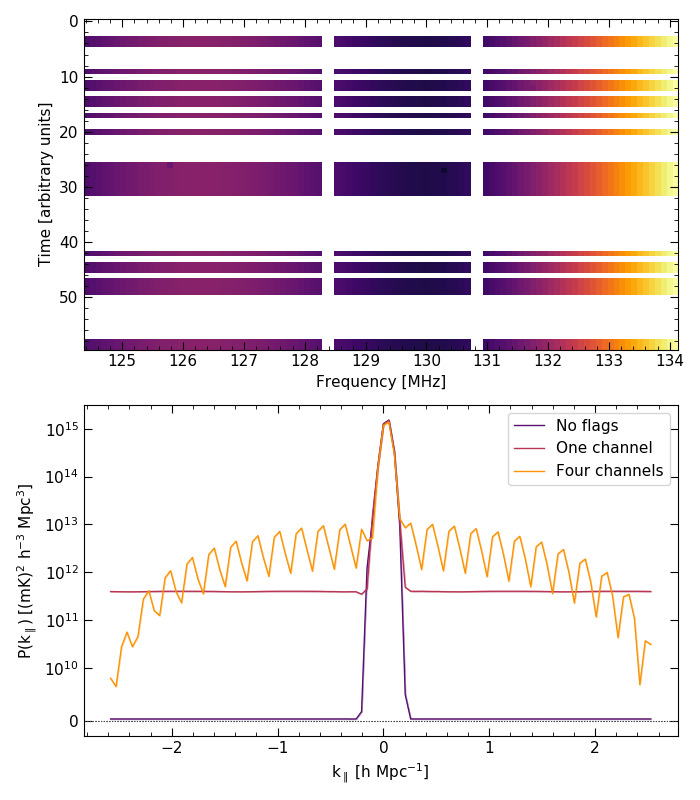
\includegraphics[width=\textwidth]{49088_sim_flag290_291_315_316.png}
	\caption[Model power spectrum calculated with flagged time integrations and four flagged channels (two blocks of two channels)]{Simulated power spectrum calculated with two blocks of two adjacent flagged channels.}
	\label{fig:sim_flag_chan290_291_315_316}
\end{figure}
\end{document}